\documentclass{article}
\usepackage[utf8]{inputenc}
\usepackage[english]{babel}
\usepackage{amsmath,amsfonts,amssymb,amsthm}
\usepackage{mathtools}
\usepackage{fancyhdr}
\usepackage{commath}
\usepackage[sc,osf]{mathpazo}
\usepackage{graphicx}
\usepackage{rotating}
\usepackage{float}
\usepackage{subcaption}
\restylefloat{table}
\usepackage{multicol}
\usepackage[dvipsnames]{xcolor}
\usepackage[colorinlistoftodos]{todonotes}
\usepackage{vmargin}  % Administrar márgenes
\setpapersize{A4} % Definir tamaño del papel
\setmargins{2.5cm} % Margen izquierdo
{1cm} % Margen superior
{16.5cm} % Área de impresión horizontal
{23.42cm} % Area de impresión vertical
{15mm} % Encabezado
{5mm} % Espacio entre el encabezado y el texto
{10pt} % Pie de página
{3mm} % Espacio entre el pie de página y el texto

\pagestyle{fancy}
\fancyhf{}
\rhead{

\includegraphics[width=4cm,height=1cm]{cropped-iitpal-at-prutor-logo.png}
}
\lhead{Determinants | Class XII}
\rfoot{}
\begin{document}
\subsection*{Example-1}
Show that,
\begin{equation*}
    \Delta=
    \begin{vmatrix}
        1 & bc & a(b+c) \\
        1 & ca & b(c+a) \\
        1 & ab & c(a+b) \\
    \end{vmatrix}
    =0
\end{equation*}
Hint: Use property 9 on column 3. Change $C_3$ as sum of $C_3$ and $C_2$.
\subsection*{Example-2}
Show that,
\begin{equation*}
    \Delta=
    \begin{vmatrix}
        1 & a & bc \\
        1 & b & ca \\
        1 & c & ab \\
    \end{vmatrix}
    =(a-b)(b-c)(c-a)
\end{equation*}
Hint: Use property 9 repeatadly on appropriate rows.
\subsection*{Example-3}
This question is based on the concept of triangle area. Lots of question have been asked from this concept in JEE Mains exam over the years. Basic concept is given as,
\begin{figure}[H]
    
    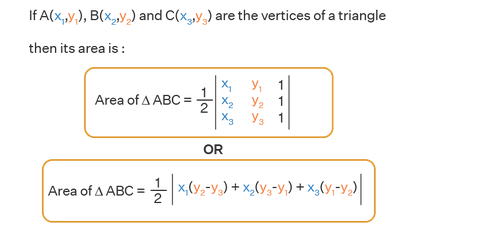
\includegraphics[scale=0.7]{determinants_lec5_exa3.png}
\end{figure}
\subsection*{Example-4 | JEE Mains 2014}

\begin{figure}[H]
    
    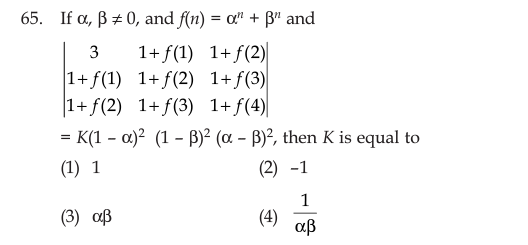
\includegraphics[scale=0.7]{determinants_lec5_exa4-que.png}
\end{figure}
\begin{figure}[H]
    % \centering
    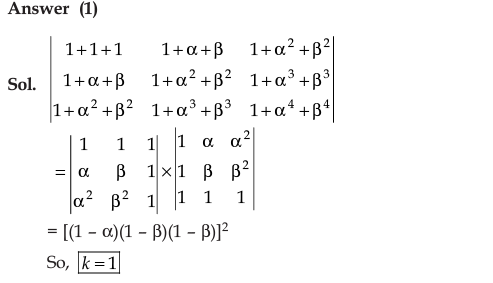
\includegraphics[scale=0.7]{determinants_lec5_exa4-ans.png}
\end{figure}
\end{document}